\documentclass{exam}
\usepackage{mainExam}

\author{Seconde 9}
\title{Vers les inéquations produits et les systèmes}
\date{27 Mai 2024}

\begin{document}
\maketitle

\section{Fonctions affines}
\begin{definitionbox}
Une \emph{fonction affine} est une fonction définie sur $\R$ de la forme $f \colon x \mapsto ax + b$, où $a$ et $b$ sont deux nombres réels. 
\begin{itemize}
\item Si $a = 0$, on dit que la fonction est \emph{constante}. 
\item Si $b = 0$, on dit que la fonction est linéaire.
\end{itemize}
\end{definitionbox}
\begin{proposition}
Soit $f$ une fonction définie sur $\R$. La courbe représentative de $f$ est une droite si et seulement si $f$ est une fonction affine.
\end{proposition}
\begin{exercize}
Relier ces différentes courbes représentatives de fonctions au fonctions correspondantes.

\begin{minipage}{0.4\textwidth}
$f \colon x \mapsto 2x + 1$

$g \colon x \mapsto -3x + 4$

$h \colon x \mapsto x$
\end{minipage}
\begin{minipage}{0.4\textwidth}
\includegraphics[width=\textwidth]{Figure3.png}
\includegraphics[width=\textwidth]{Figure2.png}
\includegraphics[width=\textwidth]{Figure1.png}
\end{minipage}
\end{exercize}
\begin{exercize}
Résoudre les équations suivantes :
\begin{enumerate}[label=\emph{\alph*)}]
\item $4x - 4 = 0$
\item $x + 3 = 0$
\item $12x - 2= 0$
\item $-7x - 14 = 0$ 
\end{enumerate}
En déduire une formule générale pour trouver l'unique antécédent de $0$ d'une fonction affine $f \colon x \mapsto ax + b$.
\end{exercize}
\newpage
\begin{exercize}
Dresser le tableau de signe des fonctions suivantes :
\begin{enumerate}[label=\emph{\alph*)}]
\item $f \colon x \mapsto -6x+3$
\item $g \colon x \mapsto 4x+3$
\end{enumerate}
En déduire les deux seuls tableaux de signes possibles pour une fonction affine quelconque.
\end{exercize}
\makeemptybox{5cm}
\section{Inequations produits}
\begin{example}
Soit l'inéquation
\begin{equation*}
(2x + 1)(x - 2) \geq 0
\end{equation*}
Pour la résoudre, il faut étudier le signe des deux fonctions $f \colon x \mapsto 2x + 1$ et $g \colon x \mapsto x - 2$.

Ces fonctions s'annulent respectivement sur $-\dfrac{1}{2}$ et $2$.

\begin{center}
\begin{tikzpicture}
\tkzTabInit[lgt=4]{$x$/1, Signe de $(2x + 1)$/1, Signe de $(x-2)$/1, Signe de $(2x+1)(x-2)$/2}{$-\infty$,$-\dfrac{1}{2}$,$2$,$+\infty$};
\tkzTabLine{,-,z,+,,+,};
\tkzTabLine{,-,,-,z,+,};
\tkzTabLine{,+,z,-,z,+,};
\end{tikzpicture}
\end{center}
Grâce au tableau de signes, on en déduit que l'ensemble des solutions est l'union d'intervalles 
\begin{equation*}
S = \left]-\infty;-\dfrac{1}{2}\right] \cup \left[2;+\infty\right[
\end{equation*}
\end{example}
\begin{exercize}
Résoudre les inéquations-produits suivantes :
\begin{enumerate}[label=\emph{\alph*)}]
\item $(x-5)(x-9)\leqslant0$
\item $(-11x-9)(-5x+9)<0$
\item $(13x+2)(3x-13)(-8x-4)\geqslant0$
\item $(x-2)(x-11)(x-12)>0$
\item $(4x+3)^2(6x-2)<0$
\item $(x-9)(x+9)\geqslant0$ 
\end{enumerate}    
\end{exercize}
\end{document}